\documentclass[12pt]{beamer}
\usetheme{Warsaw}
\usecolortheme{sidebartab}
\usefonttheme[onlysmall]{structuresmallcapsserif}
\usepackage{verbatim}
\usepackage{fancyvrb}
\usepackage{graphicx}
\usepackage{xcolor}
\usepackage[french]{babel}      
\usepackage[utf8]{inputenc}
\usepackage[T1]{fontenc}
\usepackage{url}
\usepackage{hyperref}
\usepackage{slashbox}
\usepackage{multirow}

\newcommand{\mail}[1]{\href{mailto:#1}{\nolinkurl{#1}}}

% titre [titre court] {titre long} %
\title[\LaTeX{}]{\LaTeX{}}
% Sous titre %
\subtitle {Une autre façon de faire de la Bureautique}
% autheur [autheur court ] {autheur long] %
\author[mmkmou]{Mouhamadou Moustapha CAMARA alias mmkmou}

% Institut [institut ex ecole, entreprise, ... (optionnel) ]{adresse autre infos sur l'institut} 
\institute[]{
\mail{mmkmou@gmail.com} \\
\url{http://mmkmou.legtux.org}
}

% date et lieu de la présentation [date courte] {date longue} 
\date[DAKARLUG]{11/03/2011  \\Journée de la francophonie - AUF \\ Dakar-Sénégal}

% insérer le logo 
%\logo{
\includegraphics{dakarlug}}

% début gestion des thémes et styles (css de LaTeX) %

% permet de griser les options cachées sur les tags \uncover \<+-> ... % 
\beamertemplatetransparentcovered

% définir des styles de couleurs pour le pied de page  %
\setbeamercolor*{licence}{bg=black,fg=white} % pour mettre le logo de CC 
\setbeamercolor*{shortauthor}{bg=blue!75!black,fg=white} % pour l'auteur court 
\setbeamercolor*{shorttitle}{bg=blue!75!black,fg=white} % pour le titre court
\setbeamercolor*{framenumber}{bg=black, fg=white} % pour le numéro de page
 



% modifier le template du pied de page 
\setbeamertemplate{footline}{
\leavevmode %
\hbox{%

% on définit les paramétres du premier box qui doit contenir le logo de la licence 
 \begin{beamercolorbox}[wd=.30\paperwidth,ht=2.25ex,dp=1ex,left]{licence}%
	\usebeamerfont{licence}
\includegraphics[]{image/by-nc-sa}
 \end{beamercolorbox}%

% on définit les paramétres du deuxiéme box qui doit contenir le nom court de l'autheur
 \begin{beamercolorbox}[wd=.27\paperwidth,ht=2.25ex,dp=1ex,center]{shortauthor}%
	\usebeamerfont{shortauthor}\insertshortauthor 
 \end{beamercolorbox}%

% on définit les paramétres du troisiéme box qui doit contenir le titre court :) 
 \begin{beamercolorbox}[wd=.27\paperwidth,ht=2.25ex,dp=1ex,center]{shorttitle}%
	\usebeamerfont{shorttitle}\insertshorttitle
 \end{beamercolorbox}%

% on définit les paramétres du quatriéme et dernier box qui doit contenir les numéros de page (current/total)
 \begin{beamercolorbox}[wd=.2\paperwidth,ht=2.25ex,dp=1ex,center]{framenumber}%
	\usebeamerfont{framenumber} %\insertshortdate{}\hspace*{2em}
	\insertframenumber{} / \inserttotalframenumber\hspace*{2ex}
 \end{beamercolorbox}}%




 \vskip0pt%
}

% Gérer la façon dont le plan est annoncé 

% annoncé le plan à chaque début de partie :) % 
%\AtBeginPart{\frame{\partpage}{\tableofcontents[subsectionstyle=hide]}}

% annoncé le plan à chaque début de partie :/ % 
\AtBeginSection{
	\begin{frame}<beamer>
  		\frametitle{Plan}
  		\tableofcontents[currentsection,subsectionstyle=hide]
	\end{frame}
}

% annoncé le plan à chaque sous-sections :P %
%\AtBeginSubsection[]
%{
 % \begin{frame}<beamer>
  %  \frametitle{Plan}
   % \tableofcontents[currentsection,currentsubsection]
  % \end{frame}
% }

% fin gestion des thémes et styles %

% début document % 

\begin{document}


% page de garde % 
\begin{frame}[plain]
\titlepage
\end{frame}

% slide pour les notes de licences % 

\begin{frame}[plain]
\begin{center}

\end{center}
\begin{center}

\includegraphics{image/by-nc-sa}
\end{center}
\begin{block}{Vous \^etes libres : }
\begin{itemize}
\item de reproduire, distribuer et communiquer cette création au public
\item de modifier cette création
\end{itemize}
\end{block}

\begin{block}{Selon les conditions suivantes :}
	\begin{itemize}
		\item Paternité
		\item Pas d'utilisation commerciale
		\item Partage des conditions initiales à l'identique
	\end{itemize}
\end{block}
\end{frame}

% slide introduction % 

%%%%%%%%%%%%%%%%%%%%%%%%%%%% Introduction 

\begin{frame}[plain]{Introduction}
	\LaTeX{} est : 
	\begin{enumerate}
		\item<1-> un langage;
		\item<2-> un ensemble d'outils qui permettent de composer des documents; 
		\item<3-> un ensemble de macro-commandes pour le processeur de texte \TeX{}; 
	\end{enumerate}
\end{frame}

\begin{frame}[plain]{Introduction}
	\LaTeX{} est utilisé pour rédiger : 
	\begin{enumerate}
		\item<2-> des documents scientifiques notamment en mathématique, physique et informatique;
		\item<3-> des rapports, articles, livres, slides, ...;
		\item<4-> pour faire du graphisme (dessin, couleur, schémas en 2D-3D);
		\item<5-> pour gérer une bibliographie, un index,un glossaire, ...
	\end{enumerate}
\end{frame}

%%%%%%%%%%%%%%%%%%%%%%%%%%%%% PART I
\part{Principes de base}

% \section{Environnement}
%	\begin{frame}[plain]
%		\partpage
%		\tableofcontents
%	\end{frame}

\section{Utiliser \LaTeX{}}
\begin{frame}[plain]
	Pour utiliser \LaTeX{} on a besoin de : 
	\begin{block}{}
		\begin{itemize}	
			\item<2-> Une distribution
			\item<3-> Un éditeur de texte	
		\end{itemize}
	\end{block}
\end{frame}
\subsection{Distribution}
  \begin{frame}
    Une distribution \LaTeX{} est constituée de :
    \begin{enumerate}
     \item<2-> un compilateur qui va transformer notre code en un document lisible et imprimable 
     \item<3-> un ensemble de ``packages'' pour faire des opérations plus évoluées
    \end{enumerate}
  \end{frame}
  
  \begin{frame}
   Il existe plusieurs distributions qu'on peut classer selon le systéme utilisé :
    \begin{enumerate}
     \item<2-> Mik\TeX{} et/ou Pro\TeX{} pour Windows 
     \item<3-> \TeX Live pour Unix et Gnu/Linux
     \item<4->  Mac\TeX{}  pour Mac OS
    \end{enumerate}
  \end{frame}

\subsection{Éditeur}
  \begin{frame}
  il existe plusieurs éditeurs pour \LaTeX mais les plus connus sont : 
    \begin{enumerate}
      \item<2-> \TeX nicCenter pour Windows
      \item<3-> Kile pour Gnu/Linux
      \item<4-> \TeX Shop pour MacOS
      \item<5-> \TeX Maker pour les troix OS 
    \end{enumerate}
  \end{frame}

\subsection{Installation}
  \begin{frame}
    \begin{block}{Sous Windows}
	Il faut télécharger : 
	\begin{itemize}
	 \item<2-> Pro\TeX{} -->  http://www.tug.org/protext
	 \item<3-> Mik\TeX{} -->  http://www.miktex.org
	\end{itemize}
    \end{block}
  \end{frame}

  \begin{frame}
    \begin{block}{Gnu/Linux}
      Sur certains distributions Gnu/Linux, nous avons encore Te\TeX{} dont le développement a été 
      stoppé en 2006. Nous allons utiliser \TeX live pour la suite de notre travail 
    \end{block}

    \begin{block}{}
      \begin{itemize}
	\item<2-> archive sur http://www.tug.org/texlive
	\item<3-> \verb? sudo apt-get install texlive? 
	\item<4-> \verb? sudo apt-get install texlive-latex-extra?
	\item<5-> \verb? sudo apt-get install texlive-lang-french?
	\item<6-> \verb? sudo apt-get install texlive-full?
      \end{itemize}
    \end{block}
  \end{frame}     

  
\section{Architecture}
% \begin{frame}[plain]
%  \partpage
%  \tableofcontents
% \end{frame}

\subsection{Structures}
  \begin{frame}
    \begin{block}{}
     \LaTeX est un langage de mise en page, il sert à créer des documents qui seront publiés. 
     Le fichier source LaTeX contient donc le texte ainsi que des lignes de code pour la mise 
     en page, l'insertion d'images, de tableau, ... \\
     L'idée principale est de découper la réalisation de documents en deux parties, premièrement,
     le contenu du document avec la structure : titres, chapitres, figures, tables, etc ... ensuite, 
     on ajoute dans la deuxième partie toute l'information de mise en page, les titres en gras, les 
     figures centrées, etc ...
    \end{block}
  \end{frame}

  \begin{frame}
   \includegraphics[width=11 cm,height=7 cm]{image/structure.ps}
  \end{frame}

\subsection{Cycle de production}

  \begin{frame}
    \includegraphics[width=11 cm,height=7 cm]{image/production.ps}
  \end{frame}

\subsection{Fichiers manipulés}
  \begin{frame}
	\begin{block}{}
		\begin{itemize}
			\item<2-> .tex : fichier source \TeX{} ou \LaTeX{}
			\item<3-> .sty : fichier source des extensions 
			\item<4-> .dtx, .ins : la documentation
			\item<5-> .cls : la classe d'un fichier 
		\end{itemize}
	\end{block}

	\begin{block}{}
		\begin{itemize}
			\item<6->  .dvi : fichier d'impression
			\item<7->  .log : log file
			\item<8->  .toc : tables des matiéres
			\item<9->  .lof : liste des figures
			\item<10-> .lot : liste des tableaux
			\item<11-> .aux : divers informations utiles
			\item<12-> .ind : contient l'index du document
		\end{itemize}
	\end{block}
  \end{frame}


\section{Structure des fichiers}

\subsection{Notre premier fichier \LaTeX}

	\begin{frame}[fragile]{Bonjour le monde}
		\begin{verbatim}
			\documentclass{article} 
			\usepackage[utf8]{inputenc}
			\usepackage[T1]{fontenc}
			\begin{document} 
				Bonjour le monde  
			\end{document} 
		\end{verbatim}
		\begin{block}{}
		\uncover<2-> { Dans ce texte nous pouvons distinguer deux grandes parties  :
			\begin{enumerate}
				\item<3-> Le préambule 
				\item<4-> Le corps du document 
			\end{enumerate}
		}
		\end{block}
	\end{frame}
\subsection{La classe du document}
	\begin{frame}[fragile]
		la classe du document est fourni par la commande : 
		\begin{verbatim}
			\documentclass[options1,options2,...]{classe}
		\end{verbatim}
		Pour la classe : 
		\begin{block}{}
			\begin{itemize}
				\item<2-> article --> pour un article de revue, des rapports courts
				\item<3-> book --> pour un livre  
				\item<4-> report --> pour un rapport long, thése, petit livre,... 
				\item<5-> slides -->  pour faire des transparents
				\item<6-> ...
			\end{itemize}
		\end{block}
		Pour les options :
		\begin{block}{}
			\begin{itemize}
				\item<7-> La taille de la police principale (10pt, 11pt, 12pt)
				\item<8-> La taille papier (a4paper, letterpaper,...) 
				\item<9-> type impression (twoside, oneside, twocolumn) 
			\end{itemize}
		\end{block}
	\end{frame}
\subsection{Les extensions}
	\begin{frame}[fragile]
		les extensions sont fournies par la commande : 
		\begin{verbatim}
			\usepackage[options1,options2,...]{extension}
		\end{verbatim}
		\begin{block}{}
			Le paramètre ``extension'' est le nom de l'extension à charger. On peut aussi préciser quelques options. 
			Les extensions sont gérées par votre distribution \LaTeX{} on peut en trouver sur le site de CTAN : \url{http://www.ctan.org/}
			Nous allons en voir plusieurs tout au long de notre exposé.
		\end{block}
		Exemple :
		\begin{verbatim}
			\usepackage[francais]{babel}
		\end{verbatim}
		Qui fait appel au paquet ``babel'' avec l'option ``francais''
	\end{frame}
\subsection{Les environnements}
	\begin{frame}[fragile]
		\LaTeX{} propose un ensemble d'outils sous forme d'environnements. Il s'agit d'une structure en bloc qui respecte 
		un certain nombre de régle. Sa syntaxe est la suivante : 
		\begin{verbatim}
			\begin{envi}
			 ...
			\end{envi}

		\end{verbatim}
		\texttt{envi} remplace le nom de l'environnement \\
		exple : \\
		\begin{itemize}
			\item<2-> tabbing --> pour la tabulation
			\item<3-> itemize --> pour les listes 
			\item<4-> ...
		\end{itemize}
	\end{frame}

%%%%%%%%%%%%%%%%%%%%%%%%%%% part II

\part{Mise en page du texte}

\section{Mise en page du texte}
% \begin{frame}[plain]
% \partpage
% \tableofcontents
% \end{frame}

\subsection{Structure d'un document \LaTeX{}}
	\begin{frame}[fragile]
		Il est possible d'utiliser diverses commandes pour organiser la structure de vos documents 
		logiquement. Les commandes existantes permettent de gérer les chapitres, sections, ... et 
		ces données seront entre autre utilisées lors de la génération de la table des matières.
		Ces commandes diffèrent selon la classe de document choisie
		\begin{verbatim}
			\part{title}
			\chapter{title}
			\section{title},  \subsection{title}
			\paragraph{title}, \subparagraph{title}
		\end{verbatim}
	\end{frame}
\subsection{Taille - Police}
	\begin{frame}[fragile]
		\begin{verbatim}
			\begin{tiny}
				{\normalsize Voici} ce qu'il ne faut {\Huge surtout} pas 
				faire {\Large pour {\footnotesize rendre} un texte 
				{\LARGE lisible}}
			\end{tiny}
		\end{verbatim}
		\begin{block}{}
			\begin{tiny}
				{\normalsize Voici} ce qu'il ne faut {\Huge surtout} pas faire 
				{\Large pour {\footnotesize rendre} un texte {\LARGE lisible}}
			\end{tiny}
		\end{block}
	\end{frame}
\subsection{Les Listes}
	\begin{frame}[fragile]
		\begin{verbatim}
		\begin{center}
			{\bf Travail de la semaine :}
			\begin{enumerate}
				\item Lundi
				\begin{itemize}
					\item Etudier \LaTeX
					\item RDV chez le dentiste
				\end{itemize}
				\item Mardi
				\begin{itemize}
					\item RDV chez le coiffeur
					\item Prendre ma fille chez mon ex
				\end{itemize}
			\end{enumerate}
		\end{center}
		\end{verbatim}
	\end{frame}
	\begin{frame}
		\begin{center}
			{\bf Travail de la semaine :}
			\begin{enumerate}
				\item Lundi
				\begin{itemize}
					\item Etudier \LaTeX
					\item RDV chez le dentiste
				\end{itemize}
				\item Mardi
				\begin{itemize}
					\item RDV chez le coiffeur
					\item Prendre ma fille chez mon ex
				\end{itemize}
			\end{enumerate}
		\end{center}
	\end{frame}


%%%%%%%%%%%%%%%%%%%%%%%%%%% part III
\part{Les images}
\section{Images}

% \begin{frame}[plain]
%  \partpage
%	\tableofcontents
%	\end{frame}

\subsection{Insertion}
\begin{frame}[fragile]
	\begin{block}{}
		Pour pouvoir insérer une image, il suffit d'utiliser le package graphics. 
		Une fois ce package inclus, vous pourrez utiliser la commande \verb+\includegraphics[options]{name}+ 
		qui prend comme unique paramètre le chemin de l'image à inclure.
	\end{block}
	\begin{verbatim}
		\documentclass[a4paper,11pt]{report}
			% Import des extensions
			\usepackage[utf8]{inputenc}
			\usepackage[francais]{babel}
			\usepackage{graphics}
			\begin{document}
				\includegraphics{image.eps}
			\end{document}
	\end{verbatim}
\end{frame}

\subsection{Légende}
	\begin{frame}[fragile]
		\begin{block}{}
			Pour ajouter une légende à une image, c'est assez simple, il faut utiliser l'environnement 
			figure puis utiliser la commande caption
		\end{block}
		\begin{verbatim}
			\begin{figure}
				\center
				\includegraphics[width=5cm]{image.eps}
				\caption{Superbe image}
			\end{figure}
		\end{verbatim}
	\end{frame}

%%%%%%%%%%%%%%%%%%%%%%%%% part 
\part{Tableau}

\section{Tableau}  
% \begin{frame}[plain]
% \partpage
% \tableofcontents
% \end{frame}


\subsection{tableau simple}
	\begin{frame}[fragile]
		\begin{verbatim}
			\begin{tabular}{cc}
				l 1, col 1 & l 1, col 2 \\
				l 2, col 1 & l 2, col 2 \\
			\end{tabular}
		\end{verbatim}
		\rule{\linewidth}{.5pt}  \\ 
		\begin{tabular}{cc}
			ligne 1, col 1 & ligne 1, col 2 \\
			ligne 2, col 1 & ligne 2, col 2 \\
		\end{tabular}
	\end{frame}

	\begin{frame}[fragile]
		\begin{verbatim}
			\begin{tabular}{|c|c|}
				l 1, col 1 & l 1, col 2 \\
				l 2, col 1 & l 2, col 2 \\
			\end{tabular}
		\end{verbatim}

		\begin{tabular}{|c|c|}
			\hline
			ligne 1, col 1 & ligne 1, col 2 \\
			\hline
			ligne 2, col 1 & ligne 2, col 2 \\
			\hline
		\end{tabular}
	\end{frame}
	

%%%%%%%%%%%%%%%%%%%%%%%%% End
 \part*{}
% \section{FIN}

% \subsection{remerciement} 
\begin{frame}[plain]
\begin{block}{}
\centering
Join us now and share the software \\
You'll be free hacker you'll be free
\end{block}
\end{frame}

%\subsection{Question} 
\begin{frame}[plain]
\centering
\uncover<1>{ Merci de votre attention!!!}\\
\uncover<2>{QUESTIONS ???}\\
\end{frame}

\end{document}